This chapter is aimed at introducing the reader to ForSyDe and the
goals of this thesis. 

The main intention of this introduction is to bring the reader to
understand ForSyDe in a friendly way. Thus, when necessary, clarity
was chosen over formalisms. If a complete and more accurate
description of ForSyDe is required, please refer to  \cite{forsyde} and
 \cite{forsyde:thesis}.


\section{What is ForSyDe?}

ForSyDe, which stands for \textit{Formal System Design}, is a system
design methodology \textit{``which has been developed with the
  objective to move system design to a higher level of abstraction and
  to bridge the abstraction gap by transformational design
  refinement''} \cite{forsyde:thesis}.

ForSyDe targets system modelling in general. However, by the time of
writing this thesis, the methodology only covers \textit{Synchronous
  Systems} (systems in which a global clock is used to synchronize the
different parts of the system). A well-known type of such system is
synchronous hardware, which is the main topic of the thesis.

\subsection{Why a higher abstraction level?}
The systems designed nowadays, with microelectronic systems as a
particular example, are tremendously complex due to the increasing
feature and functionality demands of the market.

Furthermore, not only designs are more complex, the aggressive
competitivity of industry requires companies to also shorten the
time-to-market of their products, affecting the development cycle.

For the reasons mentioned above, previous techniques, such as the RTL
(\textit{Register Transfer Level}) languages developed during the 80's
(mainly Verilog and VHDL) give too much detail for the designer to
handle. In other words, the level of abstraction of those techniques is
too low and hinders the design process.  As a result, a big effort was
devoted to raise the abstraction level of design automation tools,
resulting in the \textit{System-level Design} research field, to which
ForSyDe belongs.

\subsection{ForSyDe's design flow}
\begin{figure}
\centering
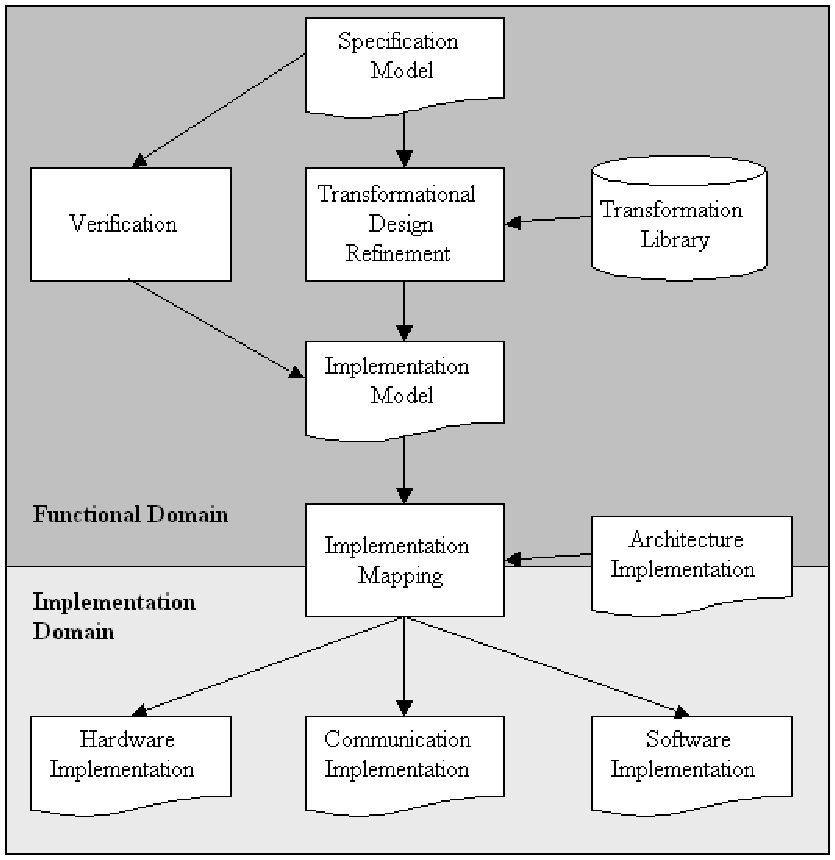
\includegraphics[width=.5\textwidth]{ForSyDeDesignFlow.pdf}
  \caption{ForSyDe's design flow}
  \label{fig:flow}
\end{figure}
\subsubsection{Specification model}
Figure \ref{fig:flow} summarizes ForSyDe's design flow. The design is
initiated by writing its \textit{specification model}.

As it was previously stated, ForSyDe currently only covers
\textit{Synchronous Systems}. For that reason, the specification model
follows a \textit{synchronous model of computation}. The
\textit{specification model} of a synchronous system in ForSyDe is
based on the concepts of \textit{synchronous signal} and
\textit{process}:

\begin{itemize}
\item A \textbf{synchronous signal} is a general term in Computer
  Science and the Telecommunications field. It can be defined as an
  entity transmitting information in a synchronous manner. That is, the
  transmission of information is arbitrated by a clock and remains
  static during each clock period, only allowed to change between
  periods. 
  
  ForSyDe uses the following notation to express a synchronous signal
  \signal{s},

  $$\overrightarrow{s} = \ll v_0,v_1,v_2,\dots \gg$$

  where $v_i$ indicates the value of the signal during period $i$ of
  the clock.
  
  From now on, this report will use the terms \textit{signal} and
  \textit{synchronous signal} equivalently.
  
\begin{figure}
\centering
\input{figures/Process.pdf_t}
  \caption{Process}
  \label{fig:proc}
\end{figure}

\item The meaning of \textit{\textbf{process}} is specific to ForSyDe
  and is represented in Figure \ref{fig:proc}.  A \textit{process} can
  be defined as a computational entity which takes $n \in
  \mathbb{N}_0$ synchronous input signals, might process them and then
  produce $m \in \mathbb{N}_0$ synchronous signals as output.
\end{itemize}
  
\begin{figure}
\centering
\input{figures/ConcurrentProcesses.pdf_t}
  \caption{A Synchronous system model in ForSyDe}
  \label{fig:concproc}
\end{figure}

A synchronous system in ForSyDe is modelled as a network of
interconnected cooperating processes which are in charge of taking the
input signals of the system, process them and finally produce its
output signals. A simplified example can be seen in figure
\ref{fig:concproc}. As a result, writing the \textit{specification
  model} consists in defining the aforementioned process
network.

The ForSyDe methodology provides a wide variety of primitive and
derived process constructors (entities used to build processes) in
which to base a model. Consult  \cite{forsyde:thesis} for details on
the available process constructors.

The following examples help to understand how the
\textit{specification model} is written and how processes
work:

\begin{figure}
\centering
\subfloat[$\mathit{mapSY}$]{
  \input{figures/mapSY.pdf_t}
  \label{fig:mapSY}
}
\subfloat[$\mathit{delaySY}$]{
  \input{figures/delaySY.pdf_t}
  \label{fig:delaySY}
}

\subfloat[$\mathit{sourceSY}$]{
  \input{figures/sourceSY.pdf_t}
  \label{fig:sourceSY}
}

  \caption{Primitive and derived process constructors}
  \label{fig:primderproc}
\end{figure}




\begin{itemize}

\item $\mathit{mapSY}$ (figure \ref{fig:mapSY}) is a primitive process
  constructor aimed at processing an input signal ($i$) through a
  function ($f$, which must be provided to the constructor in advance)
  and output it for later processing by other parts of the system.

\item The $\mathit{delaySY_k}$ primitive process constructor (figure
  \ref{fig:delaySY}), on the other hand takes an initial value $s_0$
  and delays a signal \signal{i} by $k$ clock periods

  $\mathit{delaySY_k}$ is useful to avoid zero-loops (known as
  combinational loops in the hardware world), which are not allowed in
  ForSyDe as it will be seen in next chapter.

\item $\mathit{sourceSY}$ (figure \ref{fig:sourceSY}) is a derived process
  constructor aimed at producing a custom source signal. It is derived from
  $\mathit{delaySY}$ and $\mathit{mapSY}$.

\item Figure \ref{fig:simpspec} contains a simple specification model,
  in which the reader can see its different processes. It is worth to
  note the use of numerical signals and the $\mathit{zipWithSY}_k$
  process constructor, which is a generalization of $\mathit{mapSY}$
  for $k$ inputs.
\end{itemize}


\begin{figure}
\centering
\input{figures/ConcurrentProcesses.pdf_t}
\begin{eqnarray*}
  P_1 & = & \mathit{delaySY}_1(0) \\
  P_2 & = & \mathit{zipWithSY}_2(*) \\
  P_3 & = & \mathit{zipWithSY}_2(+) \\
\end{eqnarray*}
\caption{A simple specification model}
\label{fig:simpspec}
\end{figure}

\subsubsection{Implementation model}
The next step in the design flow is to transform the specification
model into the \textit{implementation model}.

The purpose of this intermediate step is to refine the design and to
add low level information details which might be needed for an
efficient implementation. As it was stated before, ForSyDe's tries to
to \textit{``bridge the abstraction gap by transformational design
  refinement''}, which is exactly what happens in this stage.

The initial specification model is refined by automatic \textit{design
  transformation rules} which rely on the formal foundations of
ForSyDe.

Unfortunately, by the time of writing this thesis, the automatization
of this stage has not yet been implemented and constitutes a
tremendously complex task by itself due to the wide range of possible
transformations.

\subsubsection{Implementation mapping}

The last stage of the design flow consists in transforming the
\textit{implementation model} into an architecture-specific model,
such as a software implementation (e.g. C, C++, $\dots$) or hardware
specifications (e.g. VHDL,Verilog,$\dots$) from which to synthesize
hardware.


In the same way as the \textit{design transformation rules}, the
\textit{implementation mapping} stage was not automated before this
thesis was written. However, the main goal and outcome of the thesis
has been to produce a compiler to translate ForSyDe specifications
into VHDL. From the VHDL model any of the available tools can be used
to build or simulate real hardware, making possible to automatically
synthesize ForSyDe specifications.

\section{ForSyDe's implementation}
In order to use ForSyDe in practice, the designer needs a language in
which to specify the model. Current implementation of ForSyDe is based
on a EDSL (\textit{Embedded Domain Specific (programming) Language}).

\subsection{Embedded DSLs}

A DSL (\textit{Domain Specific (programming) Language}), in contrast
to a general-purpose programming language such as C, is a programming
language designed for a specific kind of task.  ForSyDe is
specifically targeted at System Modelling and for that reason, the
language chosen to write ForSyDe models must necessarily be a DSL.

On the other hand, an \textit{embedded language} is a programming
language which relies on an existing language, called \textit{host
  language}, as opposed to the embedded language itself which is
called \textit{guest language}. In practice, the guest language is
embedded by adding a library to the host language.

The main advantage of the language embedding approach is the
reutilization of the syntax of the host language, its
surrounding tools and documentation. Strongly-typed languages like
Haskell, help embedding and are a good choice as host languages due to
their encapsulation properties. However, an embedded language has, as
well, many disadvantages due to the syntactical and semantical
dependence on the host language.

Examples of popular EDSLs are YACC (the C-based parser generator) and
EmacsLisp (used as the scripting language of the popular Emacs editor).

\subsection{ForSyDe's Library}
\begin{figure}
\centering
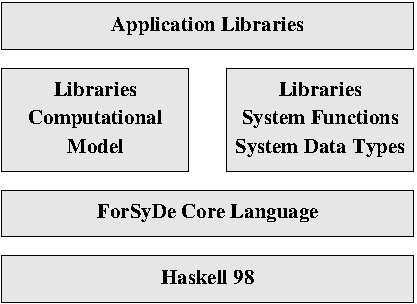
\includegraphics[width=.5\textwidth]{ForSyDeStdLib.pdf}
  \caption{ForSyDe's Library}
  \label{fig:forlib}
\end{figure}

ForSyDe is implemented as a Haskell-embedded DSL. All ForSyDe's
process constructors, together with other functionalities, are included
in a Haskell library.  Figure \ref{fig:forlib} illustrates the
structure of ForSyDe's Library which is used by the designer to write
the specification model in Haskell.

Choosing Haskell as the host language was not an arbitrary decision.
Functional languages have proven to fit nicely with hardware
design \cite{funhw}. Even if ForSyDe is aimed at system design in
general, it matches perfectly with the characteristics of Haskell:

\begin{itemize}

\item As it was previously described, a signal in ForSyDe is viewed as
  stream of values.  That makes it possible to model a signal as a list,
  which is the main data structure of functional languages in general
  and Haskell in particular.

\item Processes take signals as input, process them and output new
  signals which are later forwarded to other processes, forming a
  network. That fits perfectly well with functional languages.  A
  process can be modelled as a function which makes computations over
  lists.
  
\item The majority of ForSyDe's process constructors, such as
  $\mathit{mapSY}$, take functions as input. Yet again, that can be
  easily modelled making use of higher order functions, which are
  available in Haskell. Note that this reflects the initial intention
  of embedding ForSyDe in Haskell since its process constructors are
  named after widely-used higher-order Haskell functions (e.g.
  \texttt{map}, \texttt{zipWith} $\dots$).
\end{itemize}

During the rest of this thesis the term ForSyDe refers indistinctively
to both the methodology and its library.

\section{Thesis scope and goals}

The task of this master's thesis is to develop a tool that takes a ForSyDe
implementation model as input and produces a hardware description in VHDL.
The master's thesis must attain the following goals:

\begin{enumerate}[1)]
\item Study of ForSyDe and related work relevant to this thesis.
\item Definition of a relevant subset of Haskell that is accepted by
  the synthesis.
\item Development of the synthesis tool according to \cite{forsyde:thesis}.
\item Evaluation of the tool, identifying and including
  possible improvements.
\item Detailed documentation of the tool.
\end{enumerate}

It is important to note that it has not been possible to use the
implementation model as input due to the lack of an automatic tool to
apply the transformation rules. Instead, the compiler takes the
specification model directly. Automating the \textit{Transformational
  Design Refinement} constitutes a much larger project by itself and would have
required a high percentage of this thesis to be completed, hindering
the development of the compiler.
